\section{Preparatory Questions}

\subsection{Q1}

\begin{figure}[H]
  \begin{subfigure}{0.5\textwidth}
    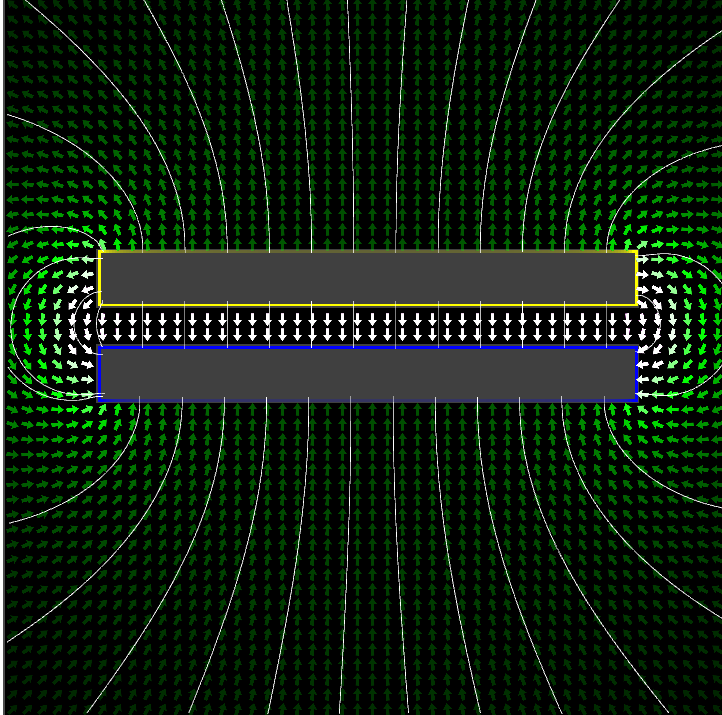
\includegraphics[width=\linewidth]{capacitors/img/small_sep.png}
    \caption{Small separation} \label{prep_answers:fig:q1:small_sep}
  \end{subfigure}
  \hspace*{\fill}
  \begin{subfigure}{0.5\textwidth}
    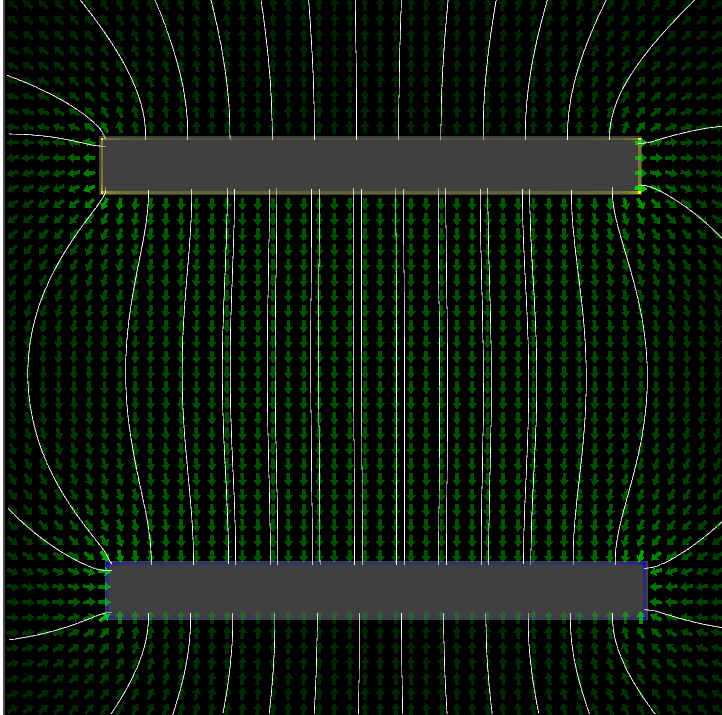
\includegraphics[width=\linewidth]{capacitors/img/large_sep.png}
    \caption{Large separation} \label{prep_answers:fig:q1:large_sep}
  \end{subfigure}
  
  \caption{The electric field for small and large separations of the capacitor plates}
  \label{prep_answers:fig:q1}
\end{figure}

From figure \ref{prep_answers:fig:q1}, the field lines inside the conducting plates are practically uniform and homogeneous. This property is enhanced when the plates are closer together. On the edges, the field lines bend, disrupting the uniformity and homogeneity. The larger the separation, the deeper the bending in the space between the two conducting plates.

\subsection{Q2}

The electrometer, used in the experiment, is sensitive even to tiny currents from minor charge redistribution due to external electric fields. If not grounded, a human body can be charged up to $1000V$ with respect to the ground resulting in an electric field which can interfere with the electrometer, effectively disrupting the measurements. If grounded, the electric potential of the body is kept $0V$ with respect to the ground, and the ground of the electrometer is also $0V$. Therefore, no external electric field will interfere with the electrometer.

However, even if grounded, it is forbidden to touch the non-insulated or non-grounded parts of the electrometer-capacitor circuit. If touched, the body acts as a conductor and a capacitor so some (capacitive) current will flow through the body, leading to false measurements.
